\documentclass[class=article, crop=false]{standalone}
\usepackage{my_preamble}
\begin{document}
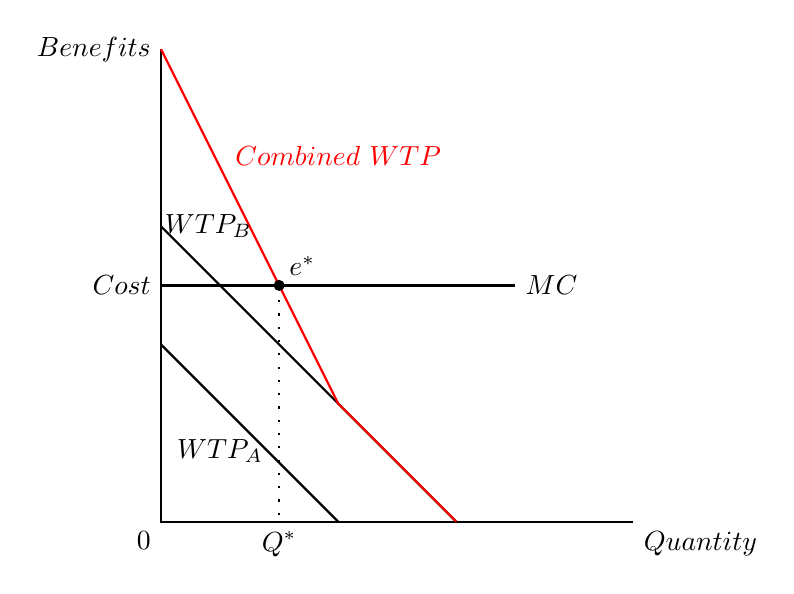
\begin{tikzpicture}[thick,font=\sffamily,scale=1.5]
	%axis
	 \draw (0,4) node[left]{$Benefits$} -- (0,0) node[below left] {$0$} -- (4,0) node[below right]{$Quantity$};
	  
	 %Graphs
	\draw[] (0,1.5) -- (1.5,0); %WTP A
	\draw[] (0,2.5) -- (2.5,0); %WTP B
	\draw[red] (0,4) -- (1.5,1) --(2.5,0); %Total WTP 
	\draw[] (0,2) -- (3,2); %MC

	%labels
	\node[red] at (1.5,3.1) {$Combined $ $WTP$}; %Total WTP label
	\node[] at (0.5,0.6) {$WTP_{A}$}; %WTP B label
	\node[] at (0.4,2.5) {$WTP_{B}$}; %WTP B label
	\node[right] at (3,2) {$MC$}; %MC label
	
	%equilibria labels
	\node[style={fill=black,circle,inner sep=0pt,minimum size=4pt}] at (1,2) { };
	\node[above right]at (1,2) {$e^{*}$};
	
	%dotted lines	
	\draw[loosely dotted] (0,2) node[left]{$Cost$} -| node[pos=0.25,below=3mm] {} (1,0) node[below]{$Q^{*}$}; %cournot dotted lines
\end{tikzpicture}
\end{document}